\subsection{Further analysis}
\label{sec:sensitivity}

\begin{figure}[!tp]
	\begin{subfigure}[]{0.995\textwidth} 
		\centering
		\caption{(a)~Gaussian mean inference~\label{fig:betas_gaussian}}
		\centering
		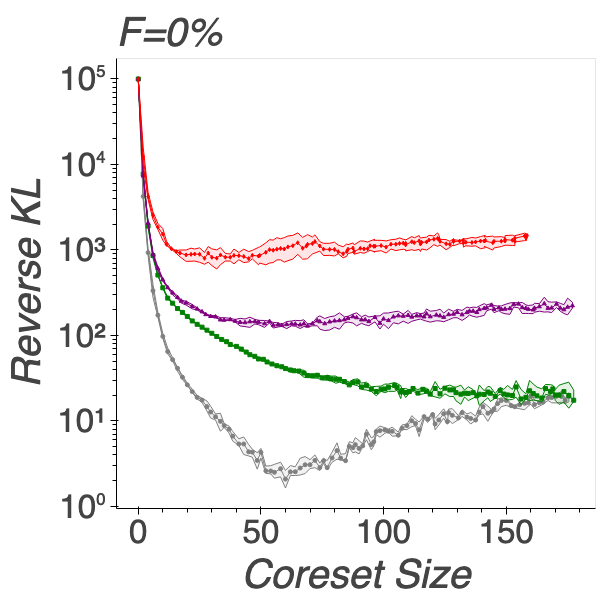
\includegraphics[width=.325\textwidth]{\MyPath/figs/comp_beta_F0_KLDvsCstSize.png}
		\centering
		\hfill
		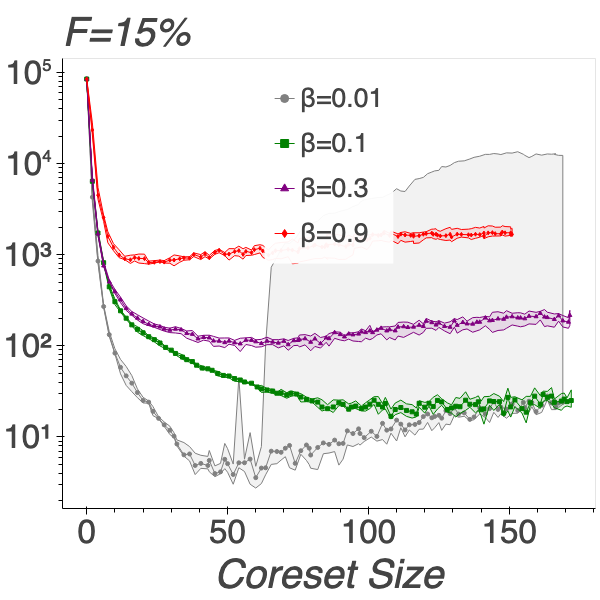
\includegraphics[width=.325\textwidth]{\MyPath/figs/comp_beta_F15_KLDvsCstSize.png}
		\centering
		\hfill
		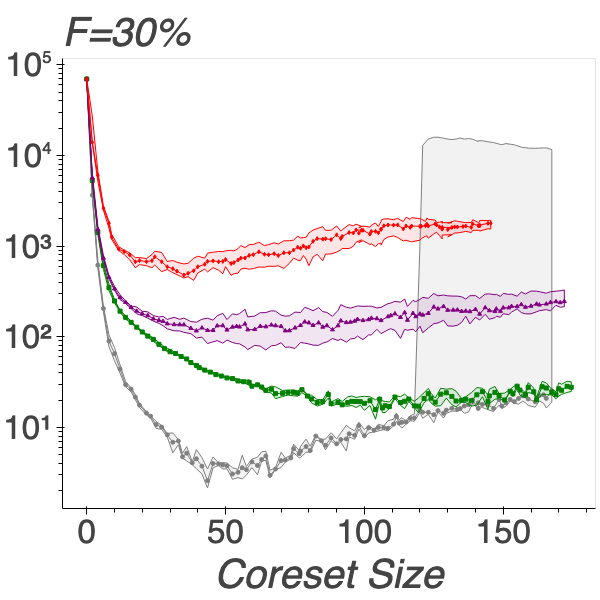
\includegraphics[width=.325\textwidth]{\MyPath/figs/comp_beta_F30_KLDvsCstSize.png}
		\centering
		\caption{(b)~Logistic regression~\label{fig:betas_logreg}}
		\centering 
		\hfill
		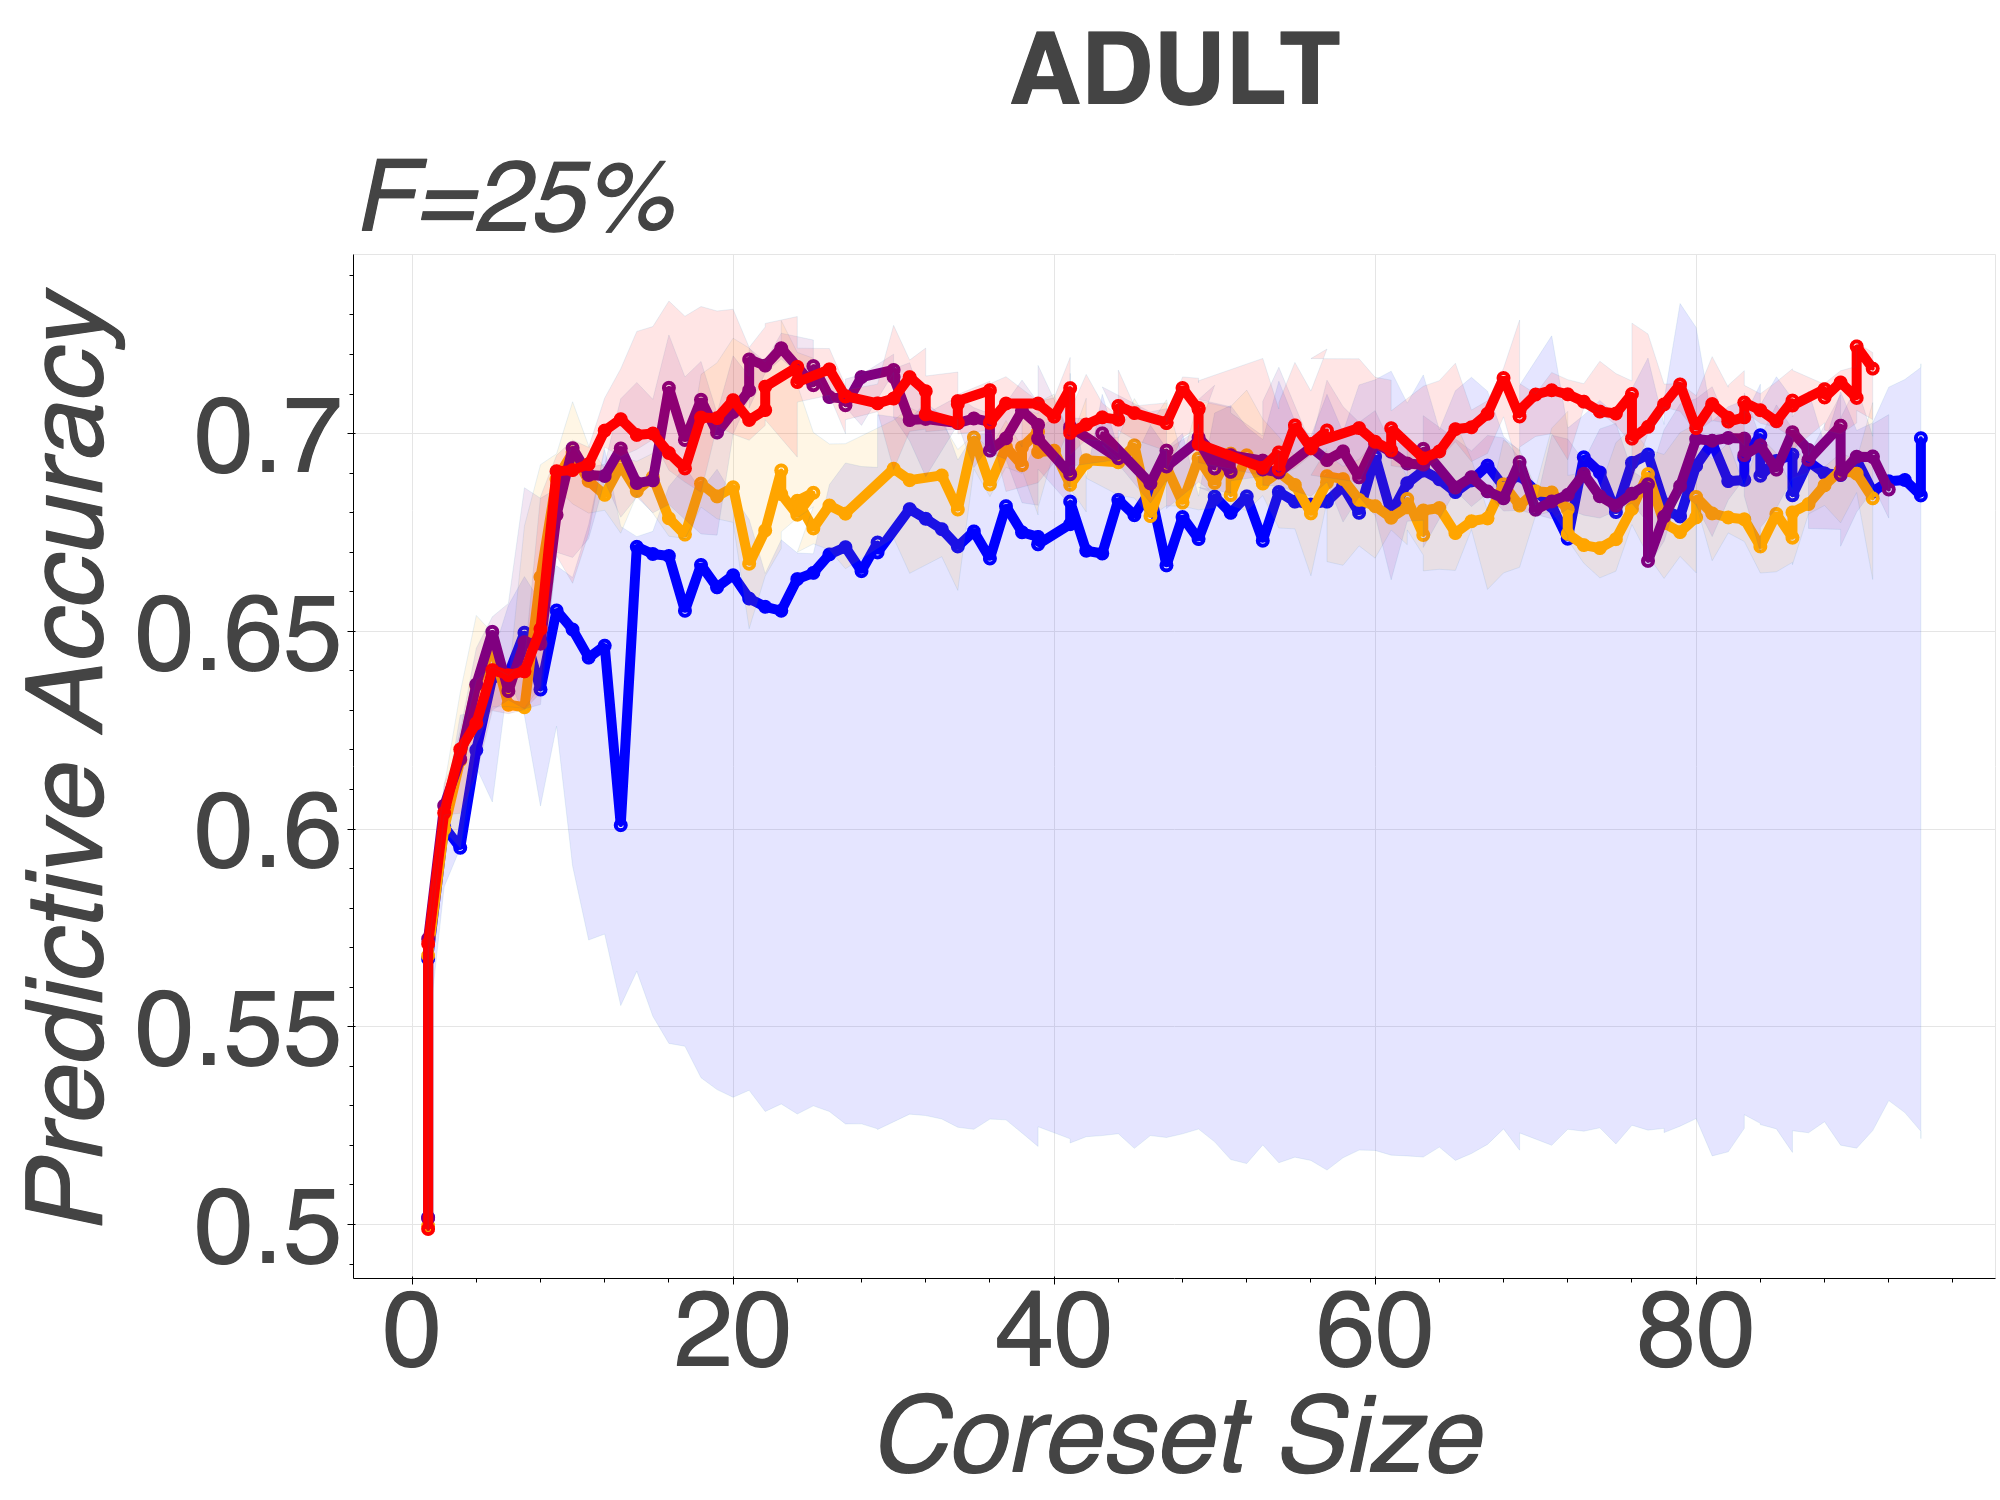
\includegraphics[width=.325\textwidth]{\MyPath/figs/comp_beta_F_25_adult_ACCvssz.png}
		\centering
		\hfil
		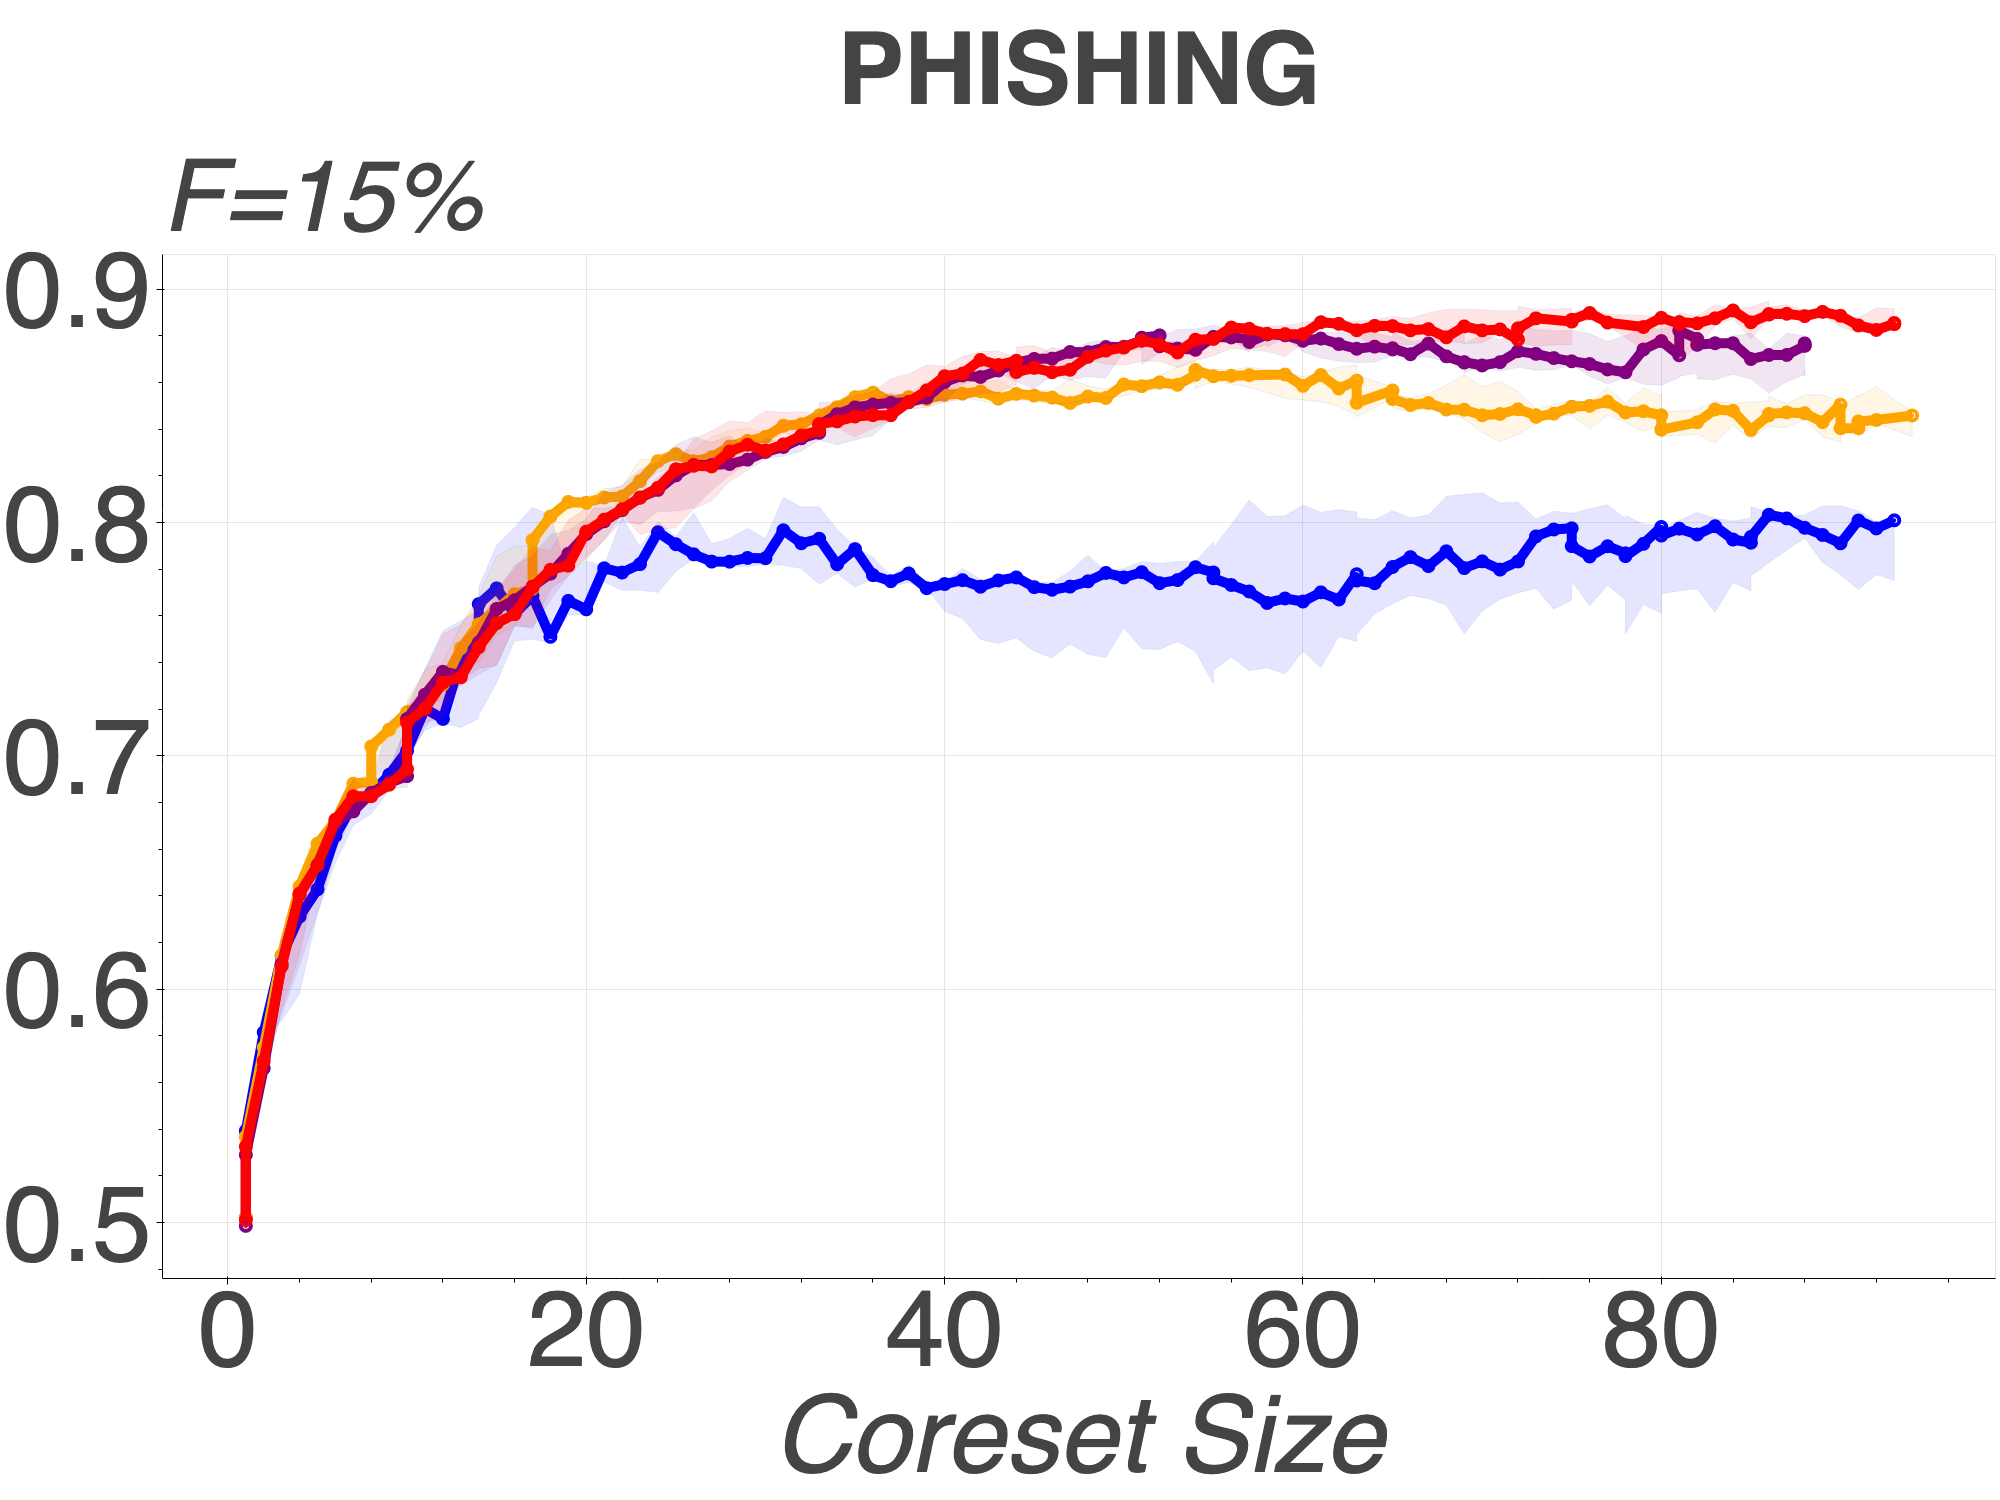
\includegraphics[width=.325\textwidth]{\MyPath/figs/comp_beta_F_15_phish_ACCvssz.png}
		\centering
		\hfill
		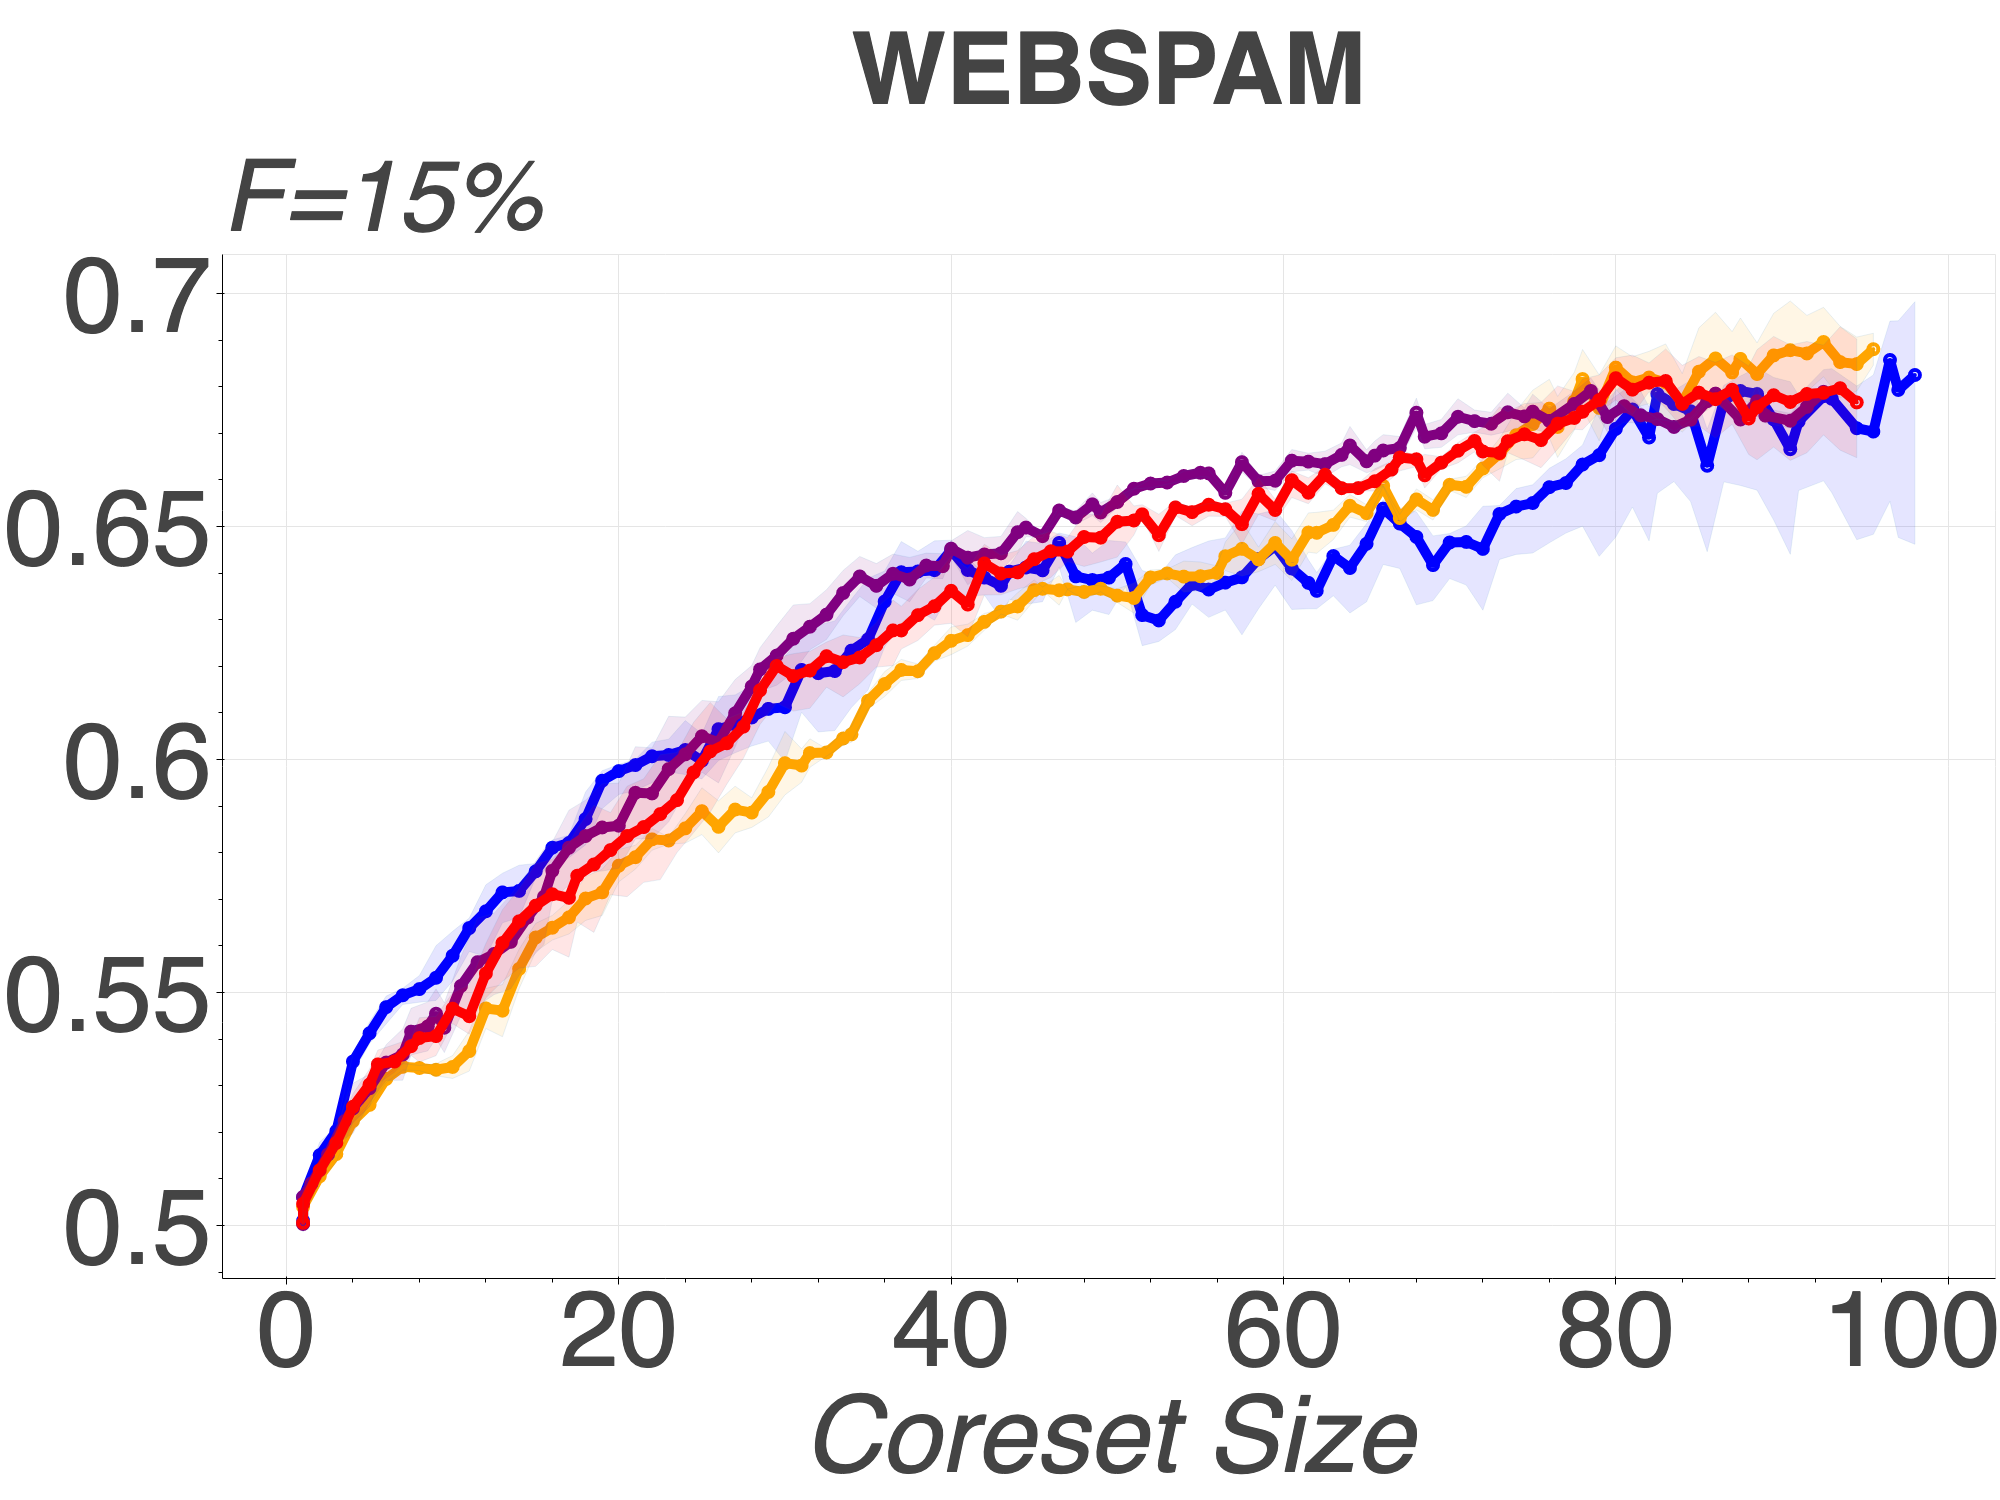
\includegraphics[width=.325\textwidth]{\MyPath/figs/comp_beta_F_15_webspam_ACCvssz.png}
		\centering
		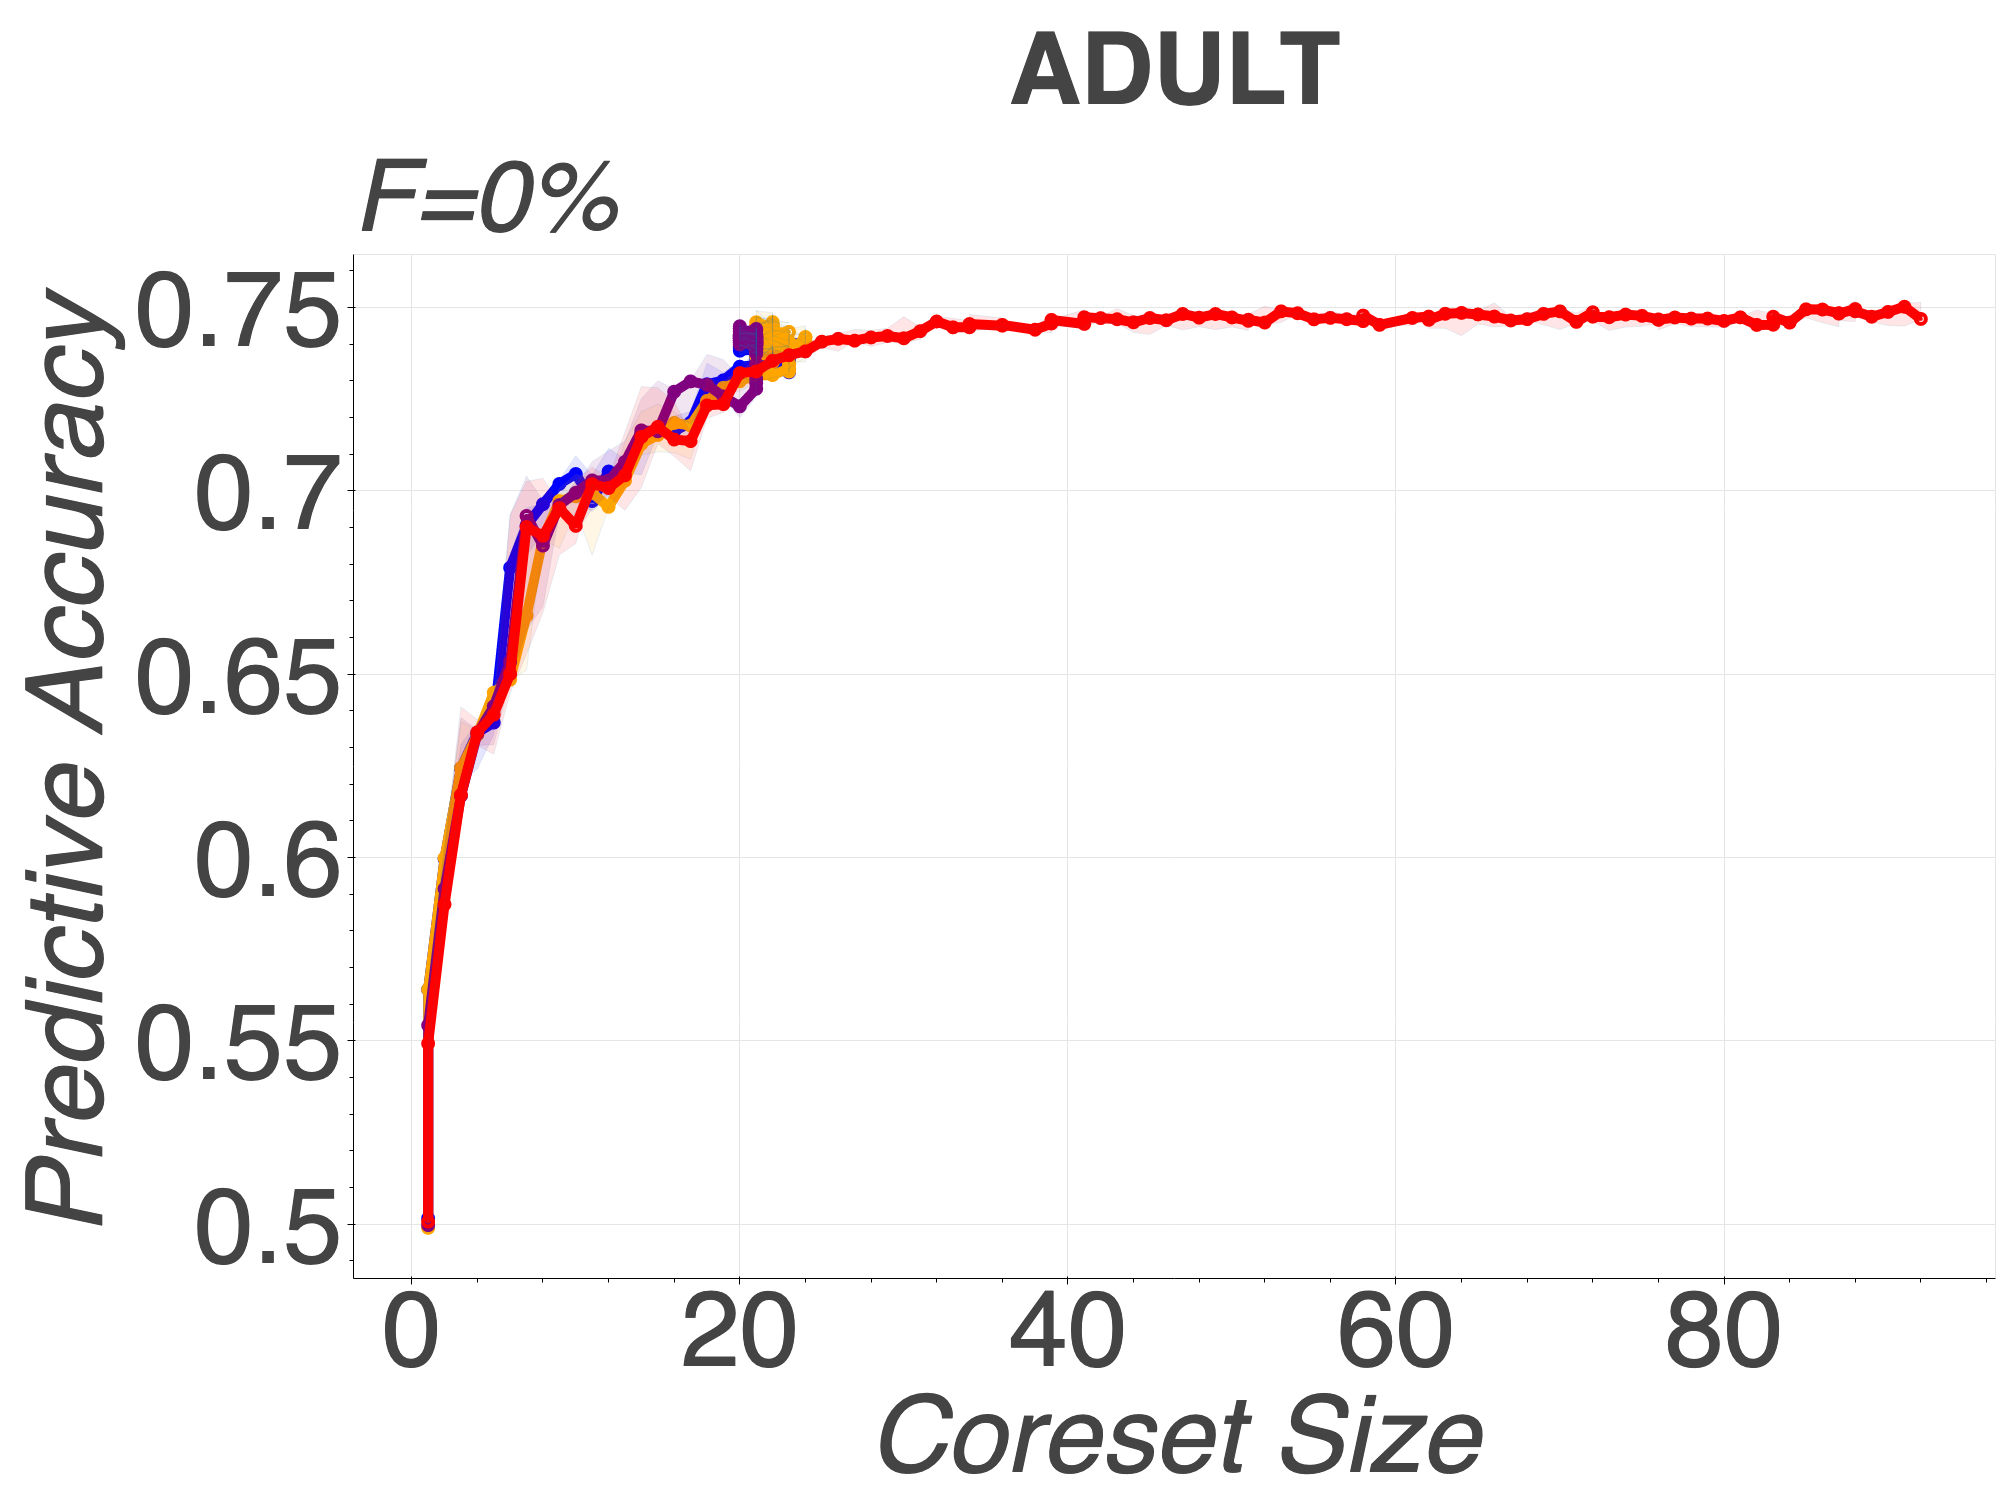
\includegraphics[width=.325\textwidth]{\MyPath/figs/comp_beta_F_0_adult_ACCvssz.png}
		\centering
		\hfill
		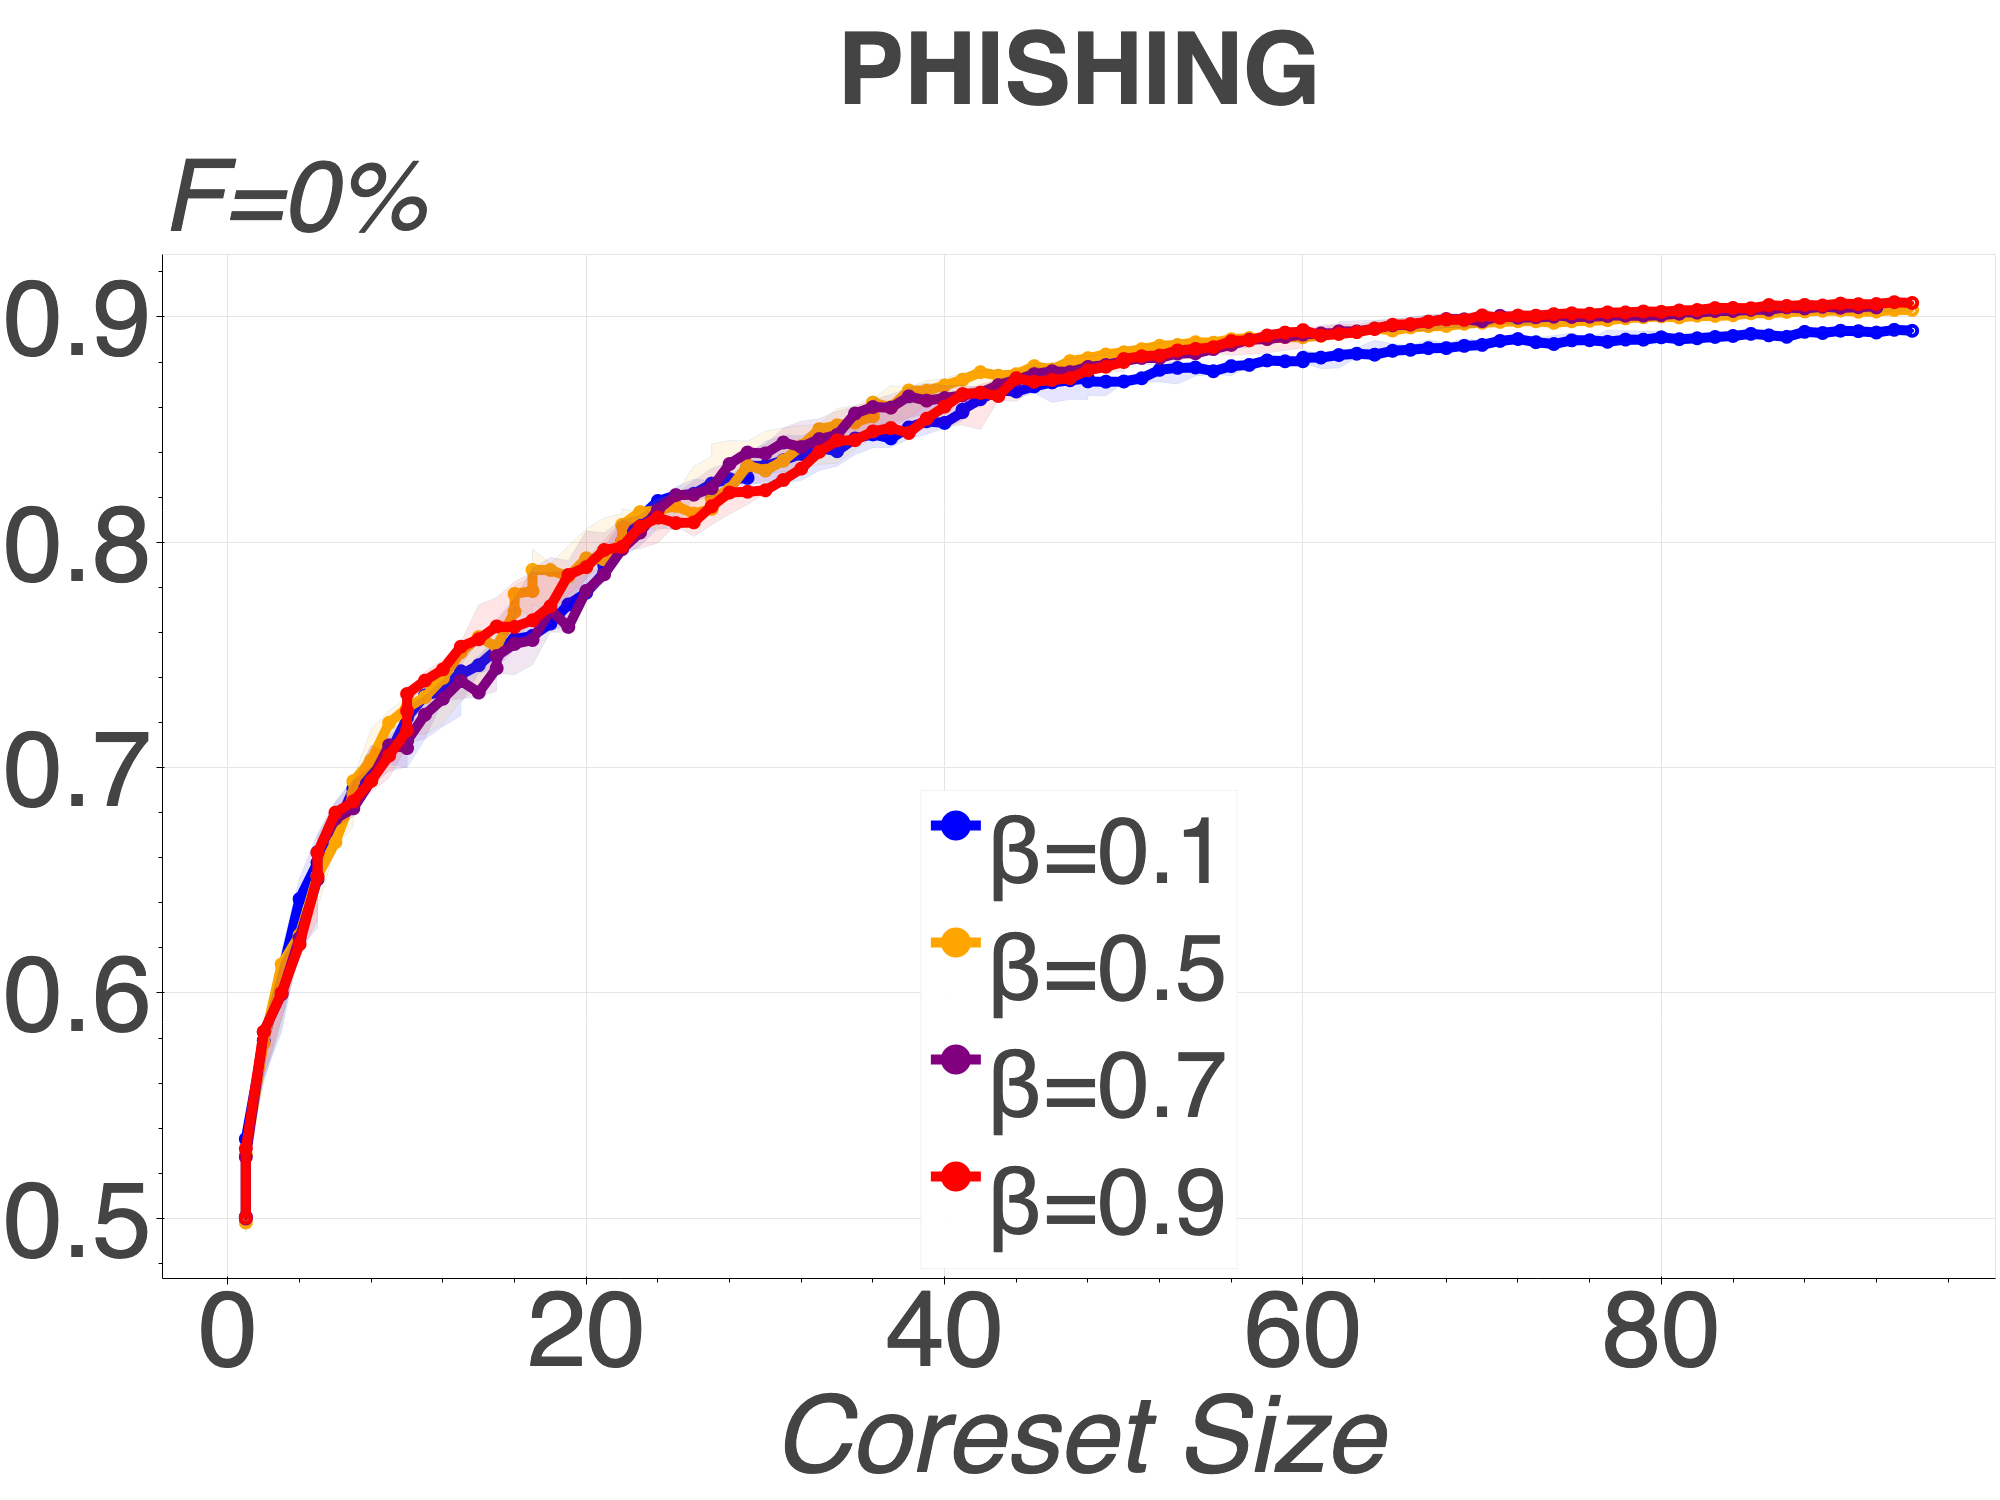
\includegraphics[width=.325\textwidth]{\MyPath/figs/comp_beta_F_0_phish_ACCvssz.png}
		\centering
		\hfill
		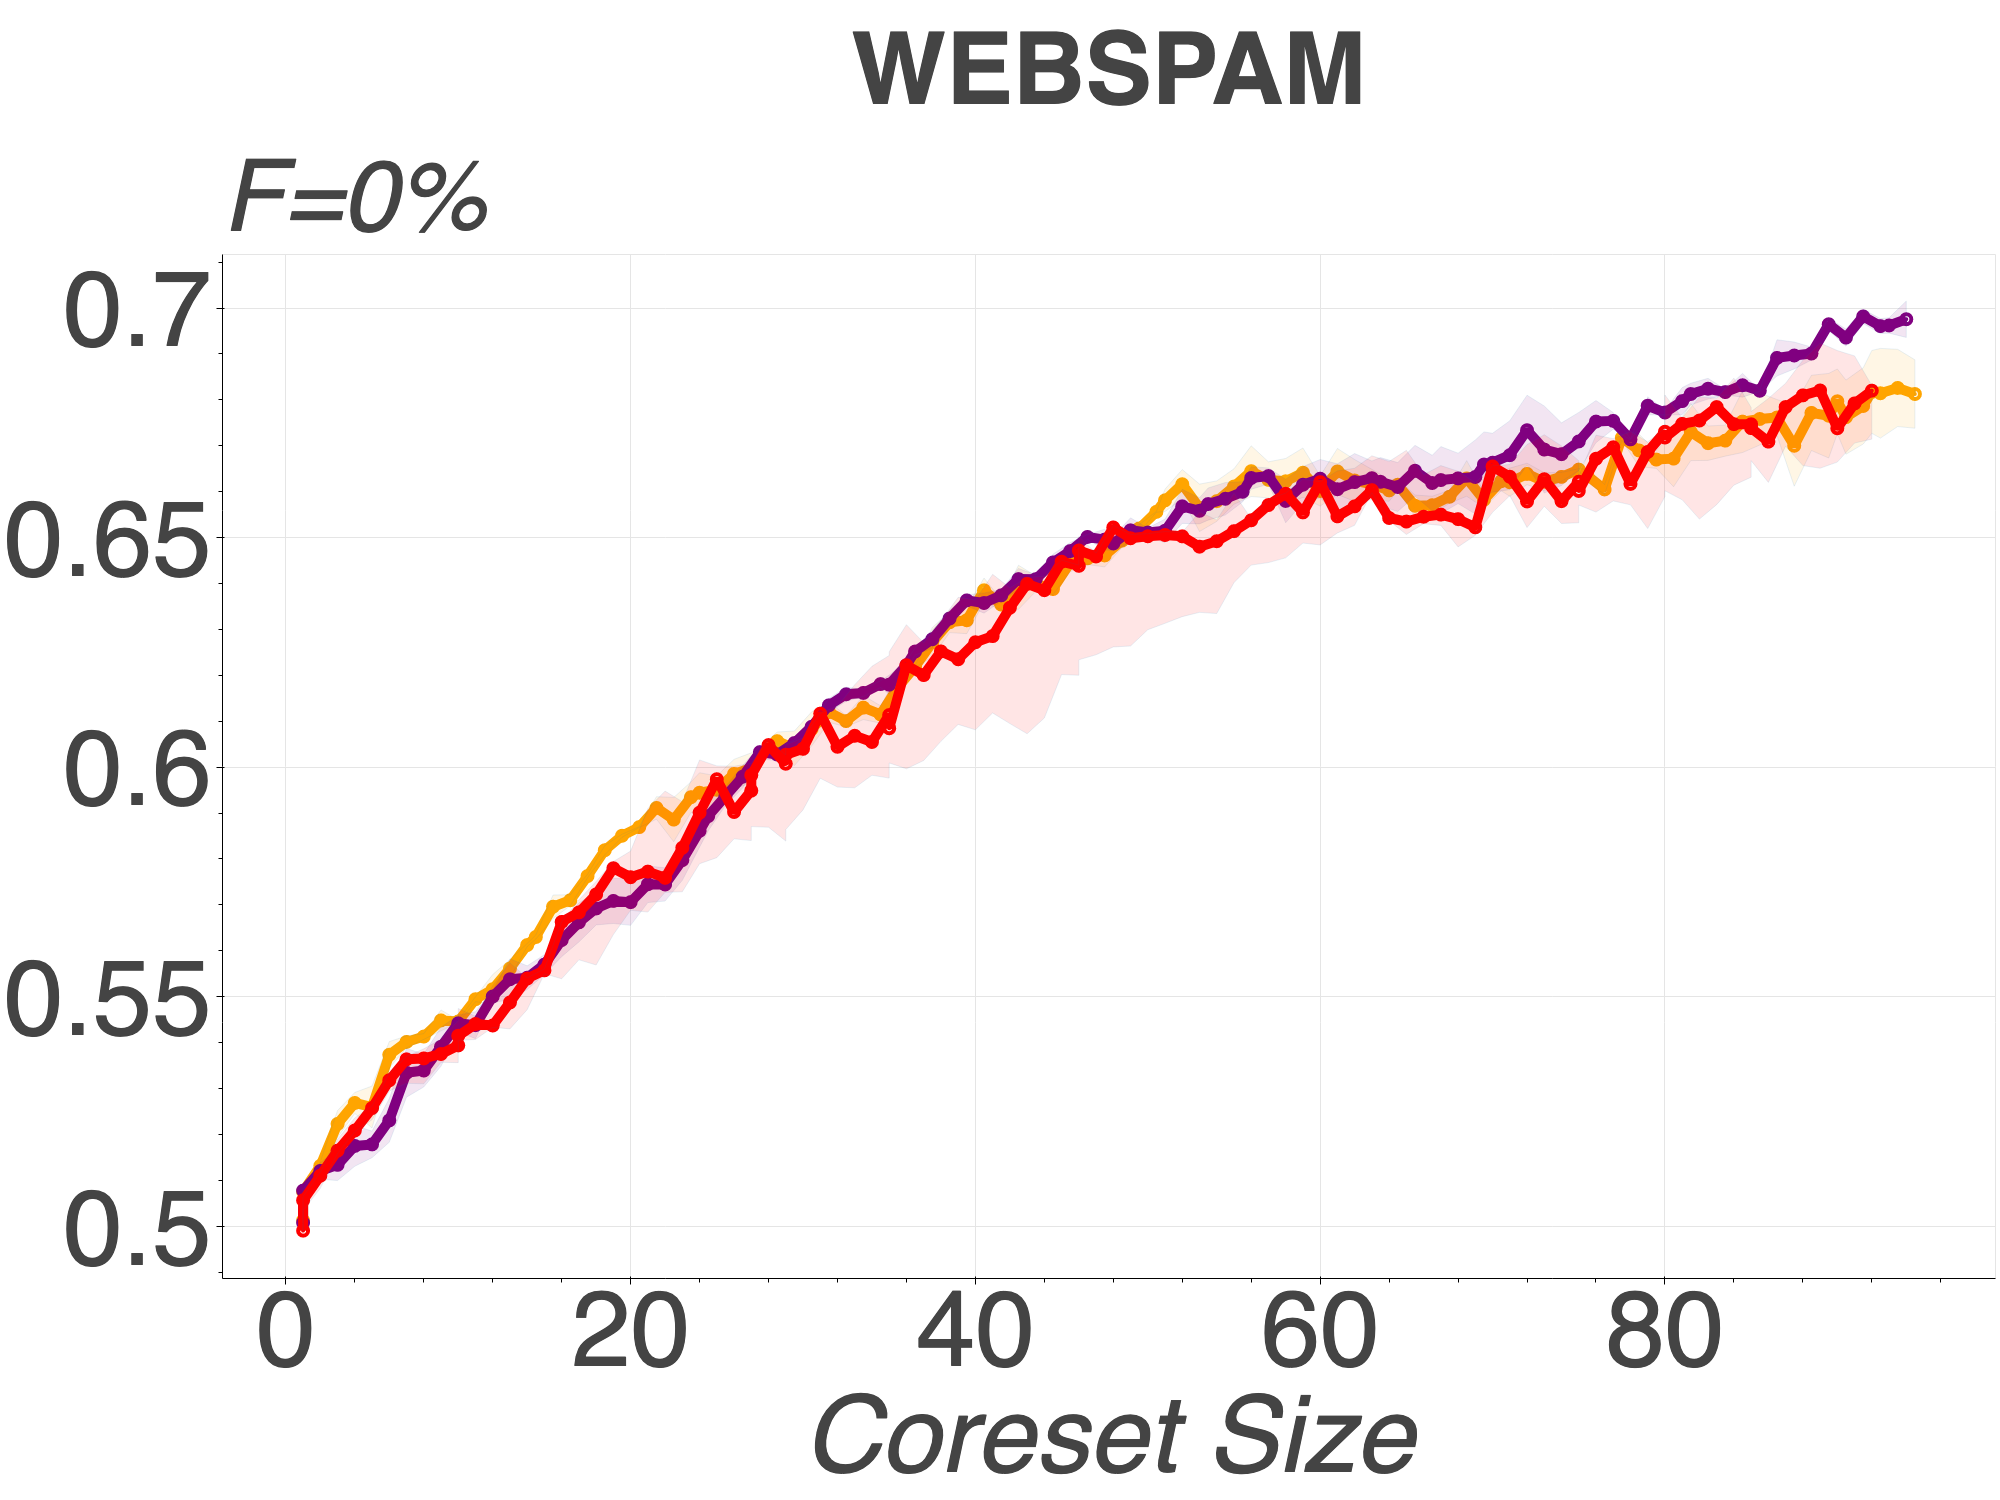
\includegraphics[width=.325\textwidth]{\MyPath/figs/comp_beta_F_0_webspam_ACCvssz.png}
		\centering
		\caption{(c)~Neural linear regression~\label{fig:betas_neurlinreg}}
		\centering
		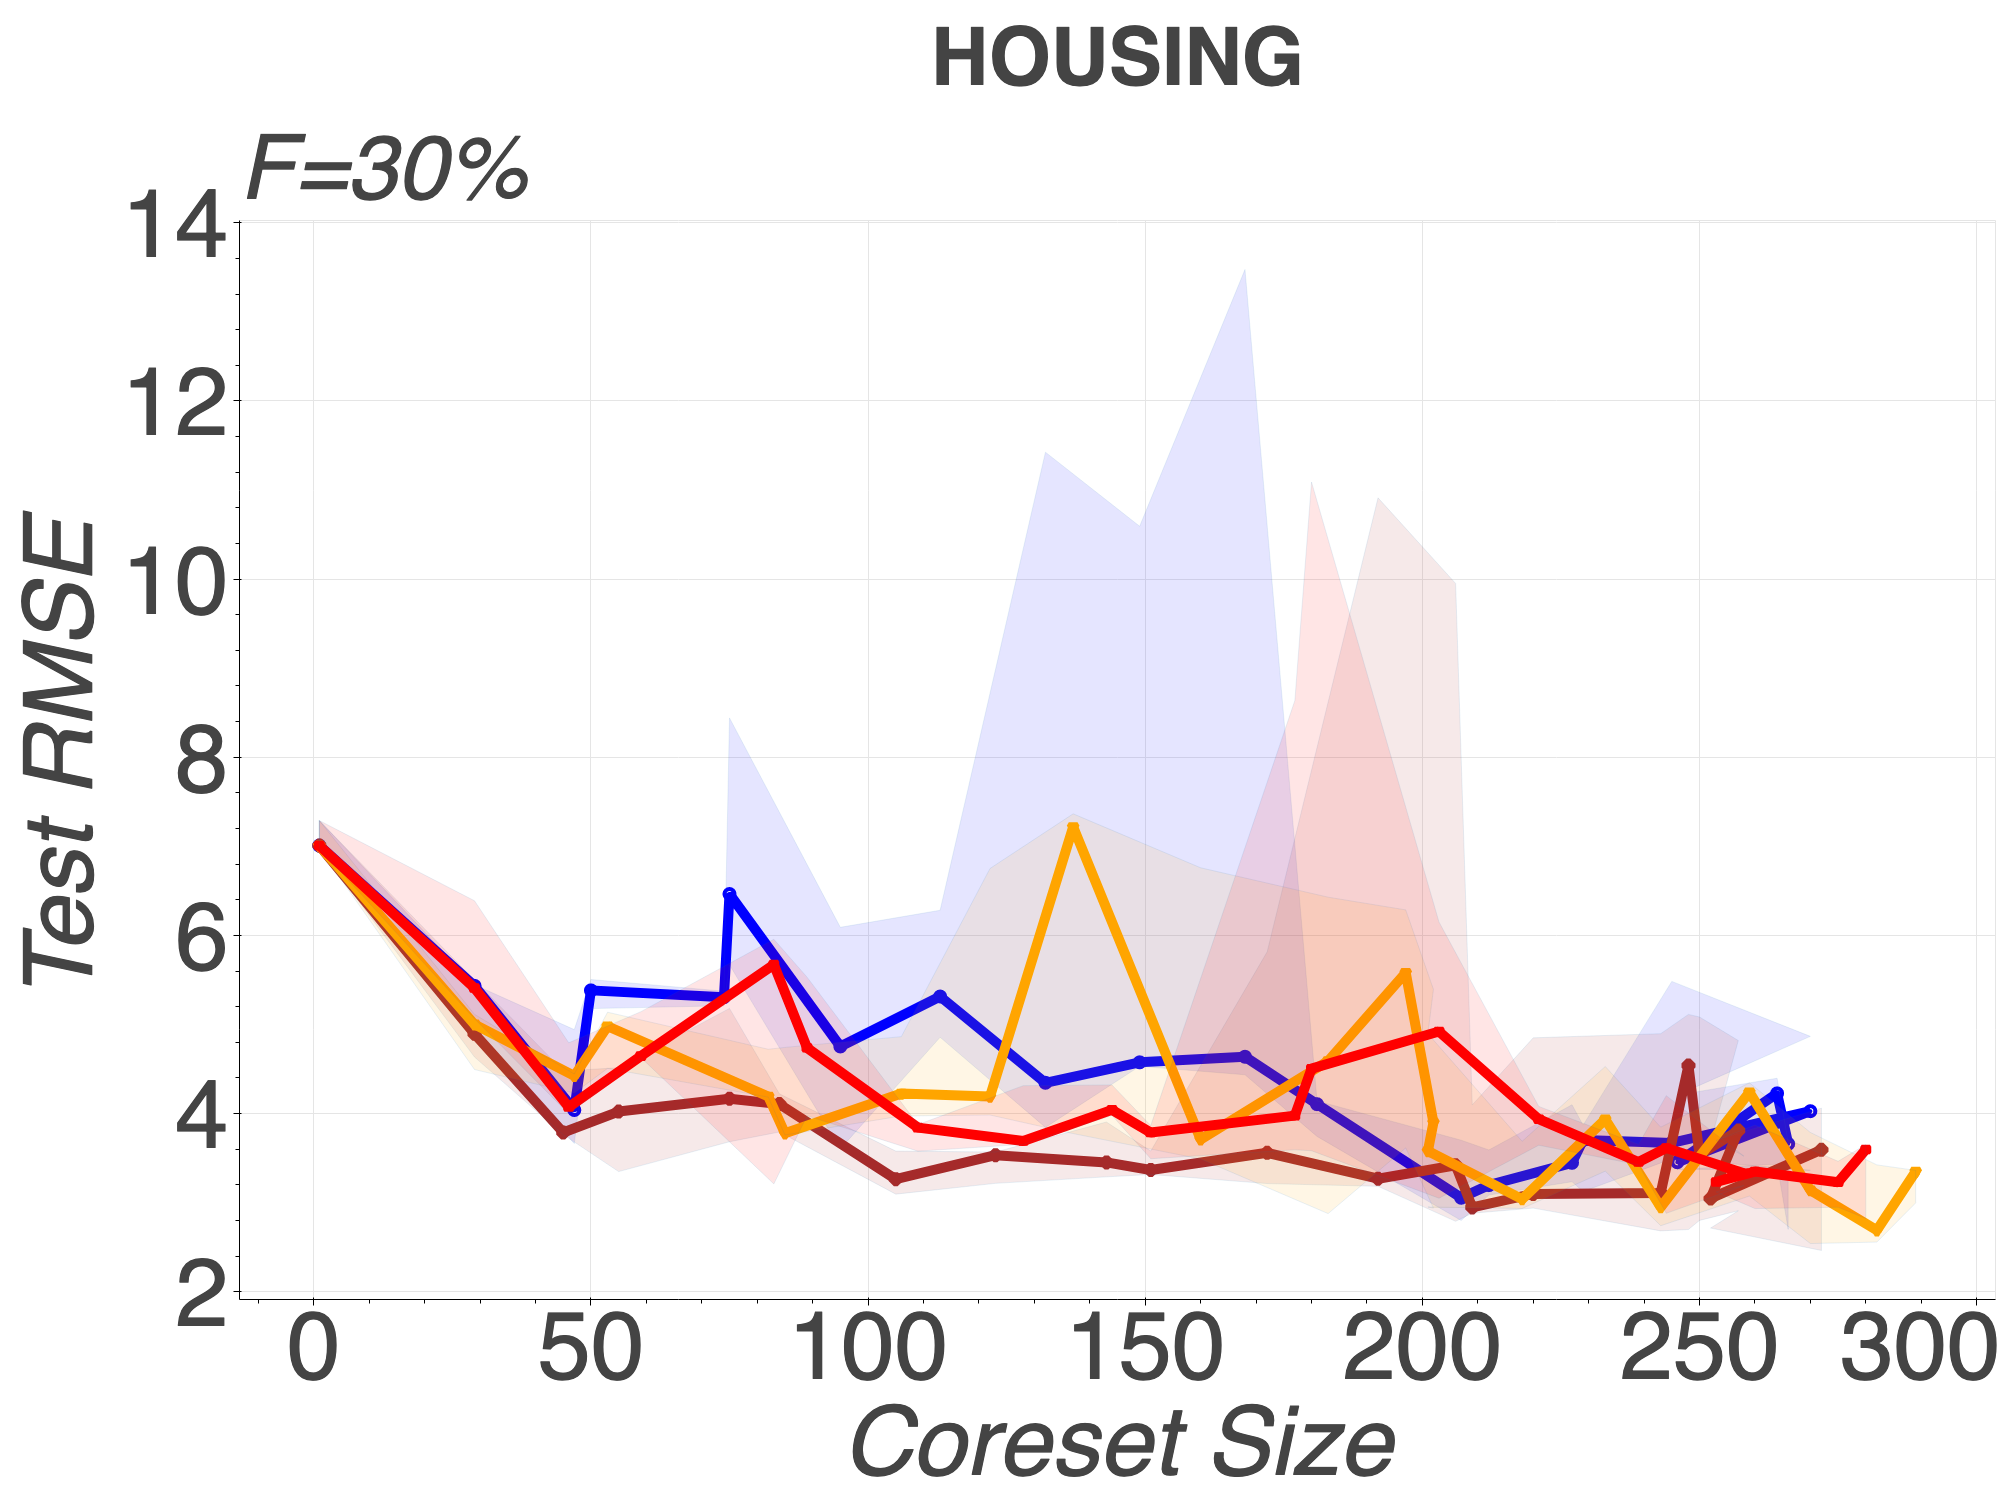
\includegraphics[width=.33\textwidth]{\MyPath/figs/comp_beta_F_boston09_01_30_RMSEvssz.png}
		\centering
		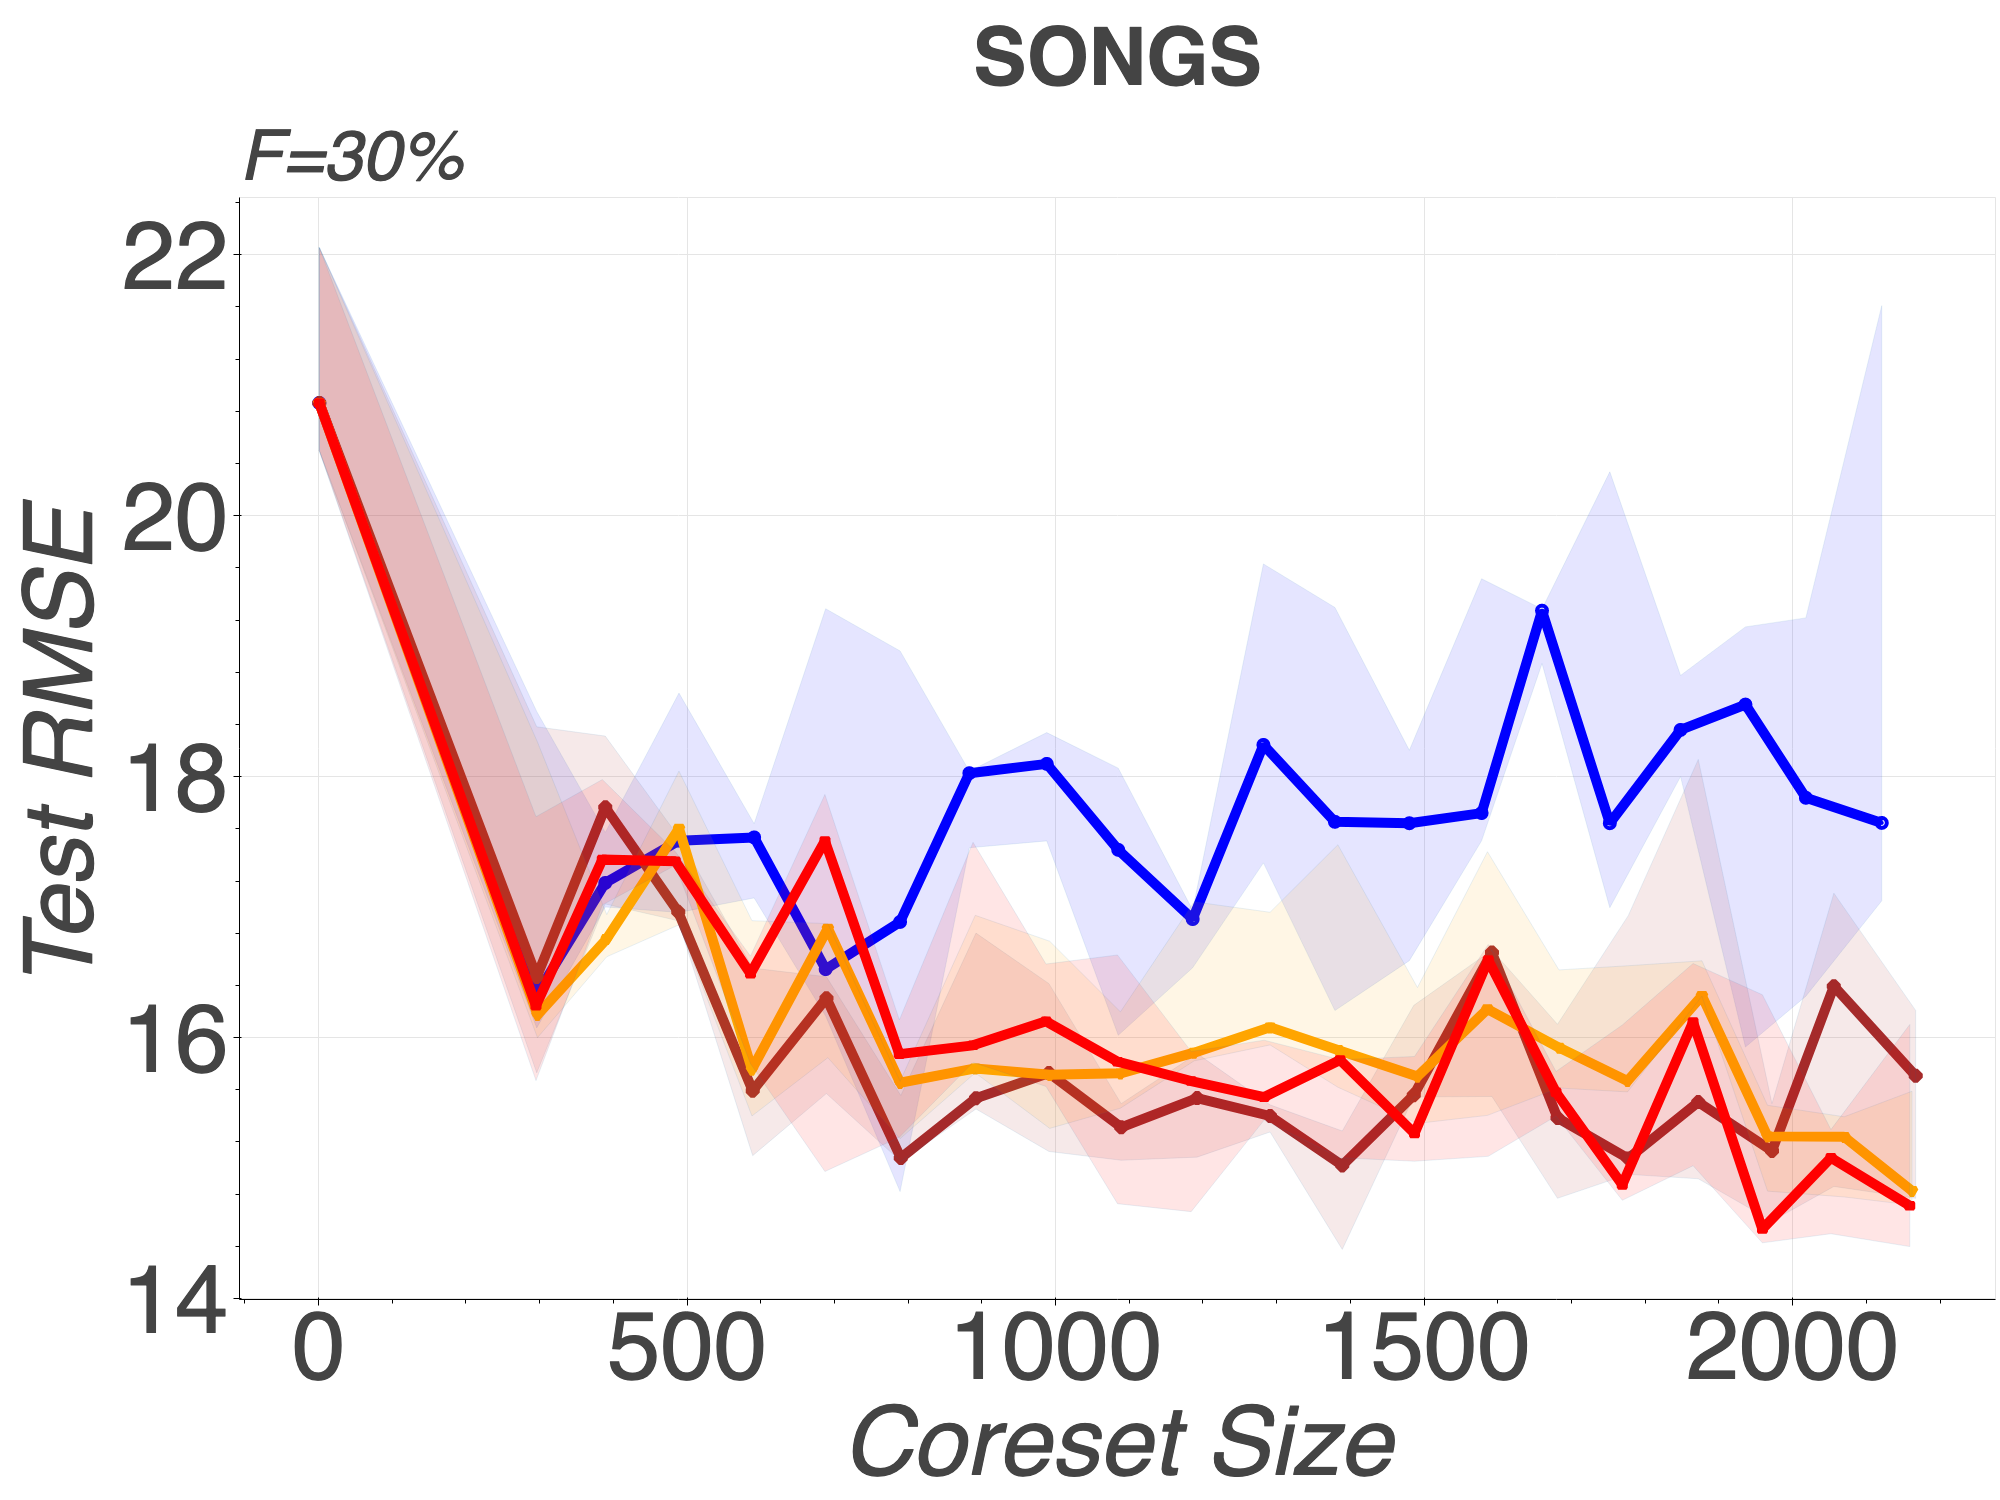
\includegraphics[width=.33\textwidth]{\MyPath/figs/comp_beta_F_year09_01_30_RMSEvssz.png}
		\centering
		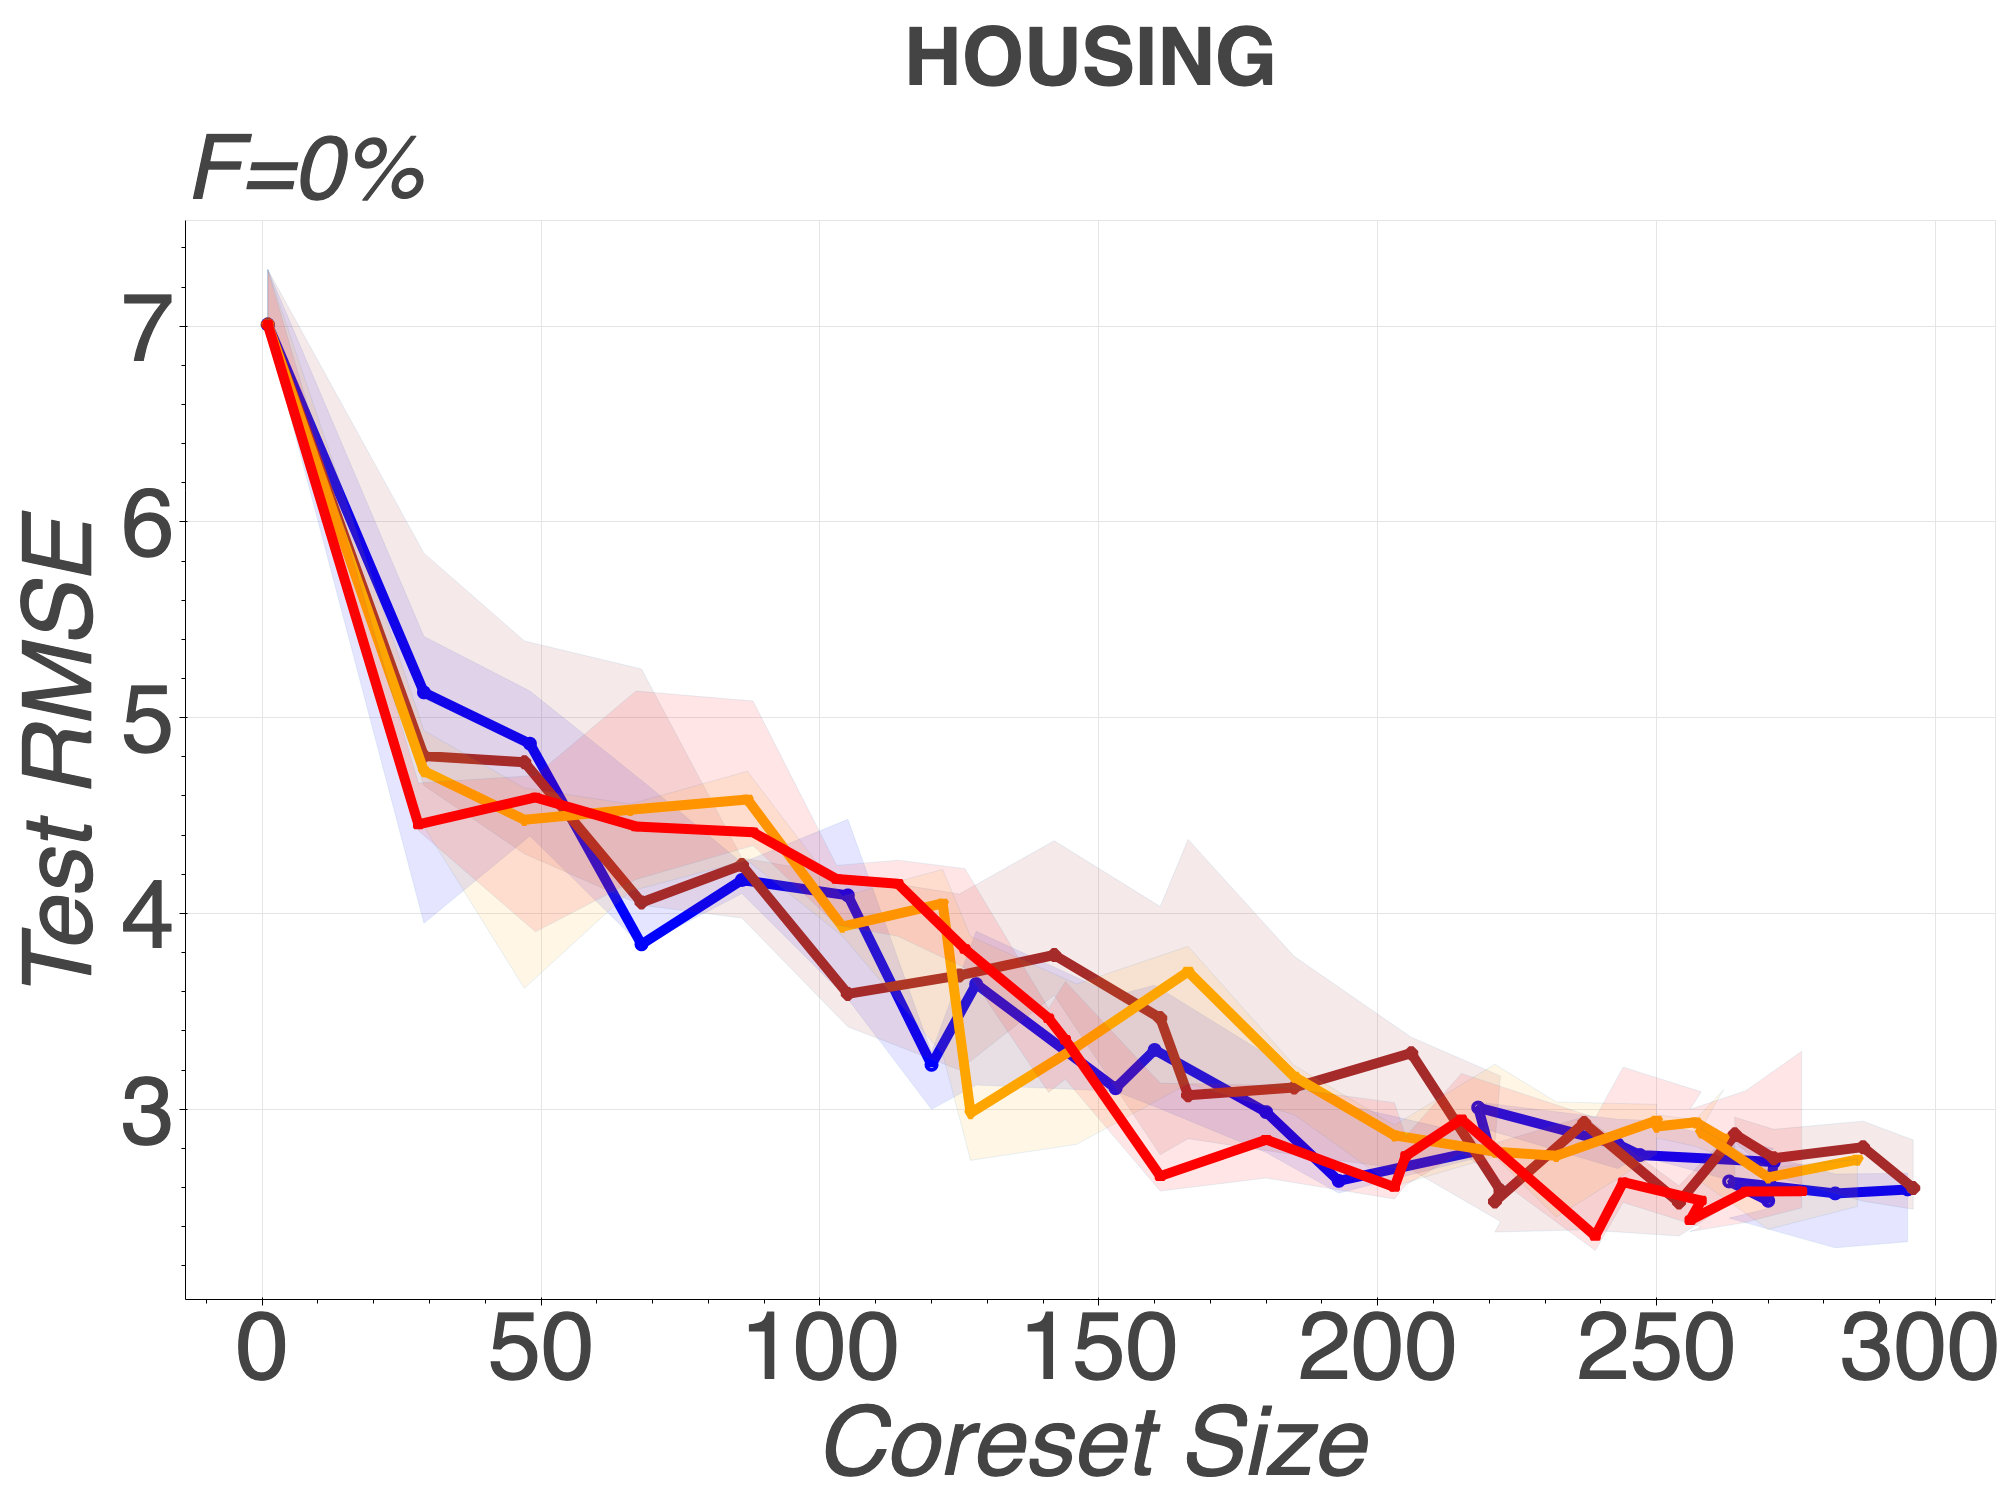
\includegraphics[width=.33\textwidth]{\MyPath/figs/comp_beta_F_boston09_01_0_RMSEvssz.png}
		\centering
		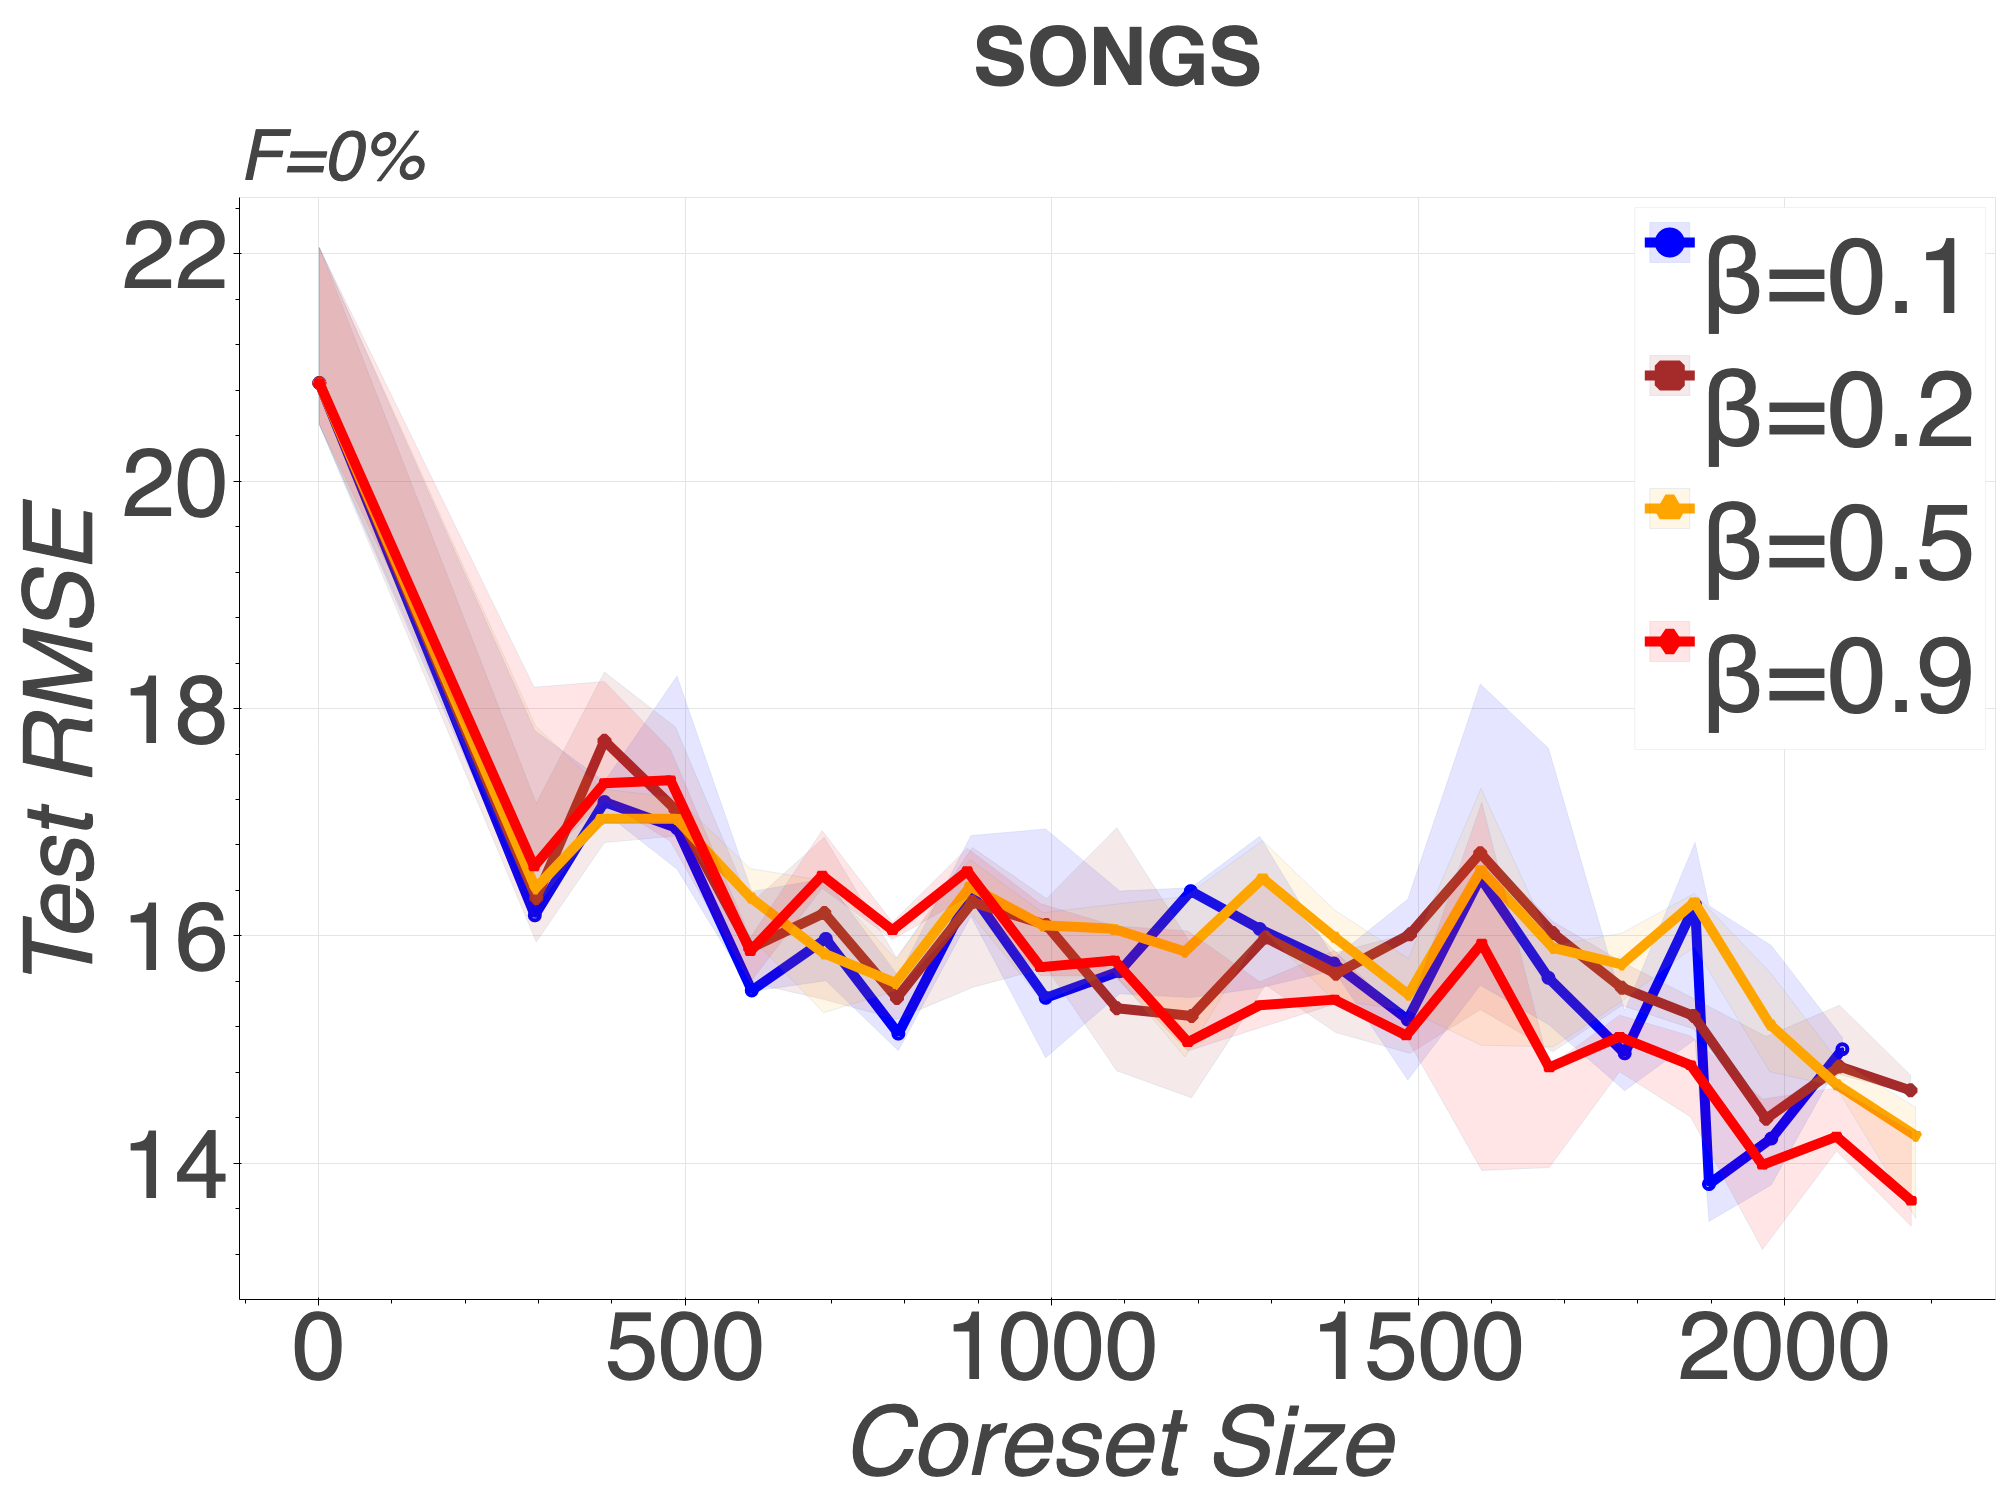
\includegraphics[width=.33\textwidth]{\MyPath/figs/comp_beta_F_year09_01_0_RMSEvssz.png}
	\end{subfigure}	
	\centering
	\caption{Predictive performance of \bcores{} for varying values of the robustness hyperparameter $\beta$. At each experiment, results are averaged over $5$ trials. Solid lines display the median of the predictive metric, with shaded areas showing the corresponding $25\textsuperscript{th}$ and $75\textsuperscript{th}$ percentiles.}
	\label{fig:beta_sens}
\end{figure}

In this section we perform an empirical analysis of the effects on robustness of inference caused by varying the value of the divergence hyperparameter $\beta \in (0,1)$. As can be observed in~\cref{fig:betas_gaussian}, in the case of Gaussian mean inference under structured contamination, setting $\beta$ to large values ($\beta \geq 0.3$) implies a more conservative summarization scheme and more rigid coreset posteriors, that do not allow good approximation quality, however maintain similar performance and small variance for increasing size of the contaminated component. For smaller $\beta$s, the KL divergence between the approximate and the true posterior can reach lower minima; nonetheless, eventually the coreset quality might present larger variance, as the summarization becomes prone to adding outliers. At the remaining experiments,~\cref{fig:betas_logreg,fig:betas_neurlinreg}, where inference takes place in the presence of unstructured outliers, the effects of varying the robustness hyperparameter are less pronounced. More noticeably, the remark of increased variance for small $\beta$ remains valid with observable effects both in the logistic and the neural linear regression experiments.


